% Options for packages loaded elsewhere
\PassOptionsToPackage{unicode}{hyperref}
\PassOptionsToPackage{hyphens}{url}
%
\documentclass[
]{book}
\usepackage{amsmath,amssymb}
\usepackage{iftex}
\ifPDFTeX
  \usepackage[T1]{fontenc}
  \usepackage[utf8]{inputenc}
  \usepackage{textcomp} % provide euro and other symbols
\else % if luatex or xetex
  \usepackage{unicode-math} % this also loads fontspec
  \defaultfontfeatures{Scale=MatchLowercase}
  \defaultfontfeatures[\rmfamily]{Ligatures=TeX,Scale=1}
\fi
\usepackage{lmodern}
\ifPDFTeX\else
  % xetex/luatex font selection
\fi
% Use upquote if available, for straight quotes in verbatim environments
\IfFileExists{upquote.sty}{\usepackage{upquote}}{}
\IfFileExists{microtype.sty}{% use microtype if available
  \usepackage[]{microtype}
  \UseMicrotypeSet[protrusion]{basicmath} % disable protrusion for tt fonts
}{}
\makeatletter
\@ifundefined{KOMAClassName}{% if non-KOMA class
  \IfFileExists{parskip.sty}{%
    \usepackage{parskip}
  }{% else
    \setlength{\parindent}{0pt}
    \setlength{\parskip}{6pt plus 2pt minus 1pt}}
}{% if KOMA class
  \KOMAoptions{parskip=half}}
\makeatother
\usepackage{xcolor}
\usepackage{color}
\usepackage{fancyvrb}
\newcommand{\VerbBar}{|}
\newcommand{\VERB}{\Verb[commandchars=\\\{\}]}
\DefineVerbatimEnvironment{Highlighting}{Verbatim}{commandchars=\\\{\}}
% Add ',fontsize=\small' for more characters per line
\usepackage{framed}
\definecolor{shadecolor}{RGB}{248,248,248}
\newenvironment{Shaded}{\begin{snugshade}}{\end{snugshade}}
\newcommand{\AlertTok}[1]{\textcolor[rgb]{0.94,0.16,0.16}{#1}}
\newcommand{\AnnotationTok}[1]{\textcolor[rgb]{0.56,0.35,0.01}{\textbf{\textit{#1}}}}
\newcommand{\AttributeTok}[1]{\textcolor[rgb]{0.13,0.29,0.53}{#1}}
\newcommand{\BaseNTok}[1]{\textcolor[rgb]{0.00,0.00,0.81}{#1}}
\newcommand{\BuiltInTok}[1]{#1}
\newcommand{\CharTok}[1]{\textcolor[rgb]{0.31,0.60,0.02}{#1}}
\newcommand{\CommentTok}[1]{\textcolor[rgb]{0.56,0.35,0.01}{\textit{#1}}}
\newcommand{\CommentVarTok}[1]{\textcolor[rgb]{0.56,0.35,0.01}{\textbf{\textit{#1}}}}
\newcommand{\ConstantTok}[1]{\textcolor[rgb]{0.56,0.35,0.01}{#1}}
\newcommand{\ControlFlowTok}[1]{\textcolor[rgb]{0.13,0.29,0.53}{\textbf{#1}}}
\newcommand{\DataTypeTok}[1]{\textcolor[rgb]{0.13,0.29,0.53}{#1}}
\newcommand{\DecValTok}[1]{\textcolor[rgb]{0.00,0.00,0.81}{#1}}
\newcommand{\DocumentationTok}[1]{\textcolor[rgb]{0.56,0.35,0.01}{\textbf{\textit{#1}}}}
\newcommand{\ErrorTok}[1]{\textcolor[rgb]{0.64,0.00,0.00}{\textbf{#1}}}
\newcommand{\ExtensionTok}[1]{#1}
\newcommand{\FloatTok}[1]{\textcolor[rgb]{0.00,0.00,0.81}{#1}}
\newcommand{\FunctionTok}[1]{\textcolor[rgb]{0.13,0.29,0.53}{\textbf{#1}}}
\newcommand{\ImportTok}[1]{#1}
\newcommand{\InformationTok}[1]{\textcolor[rgb]{0.56,0.35,0.01}{\textbf{\textit{#1}}}}
\newcommand{\KeywordTok}[1]{\textcolor[rgb]{0.13,0.29,0.53}{\textbf{#1}}}
\newcommand{\NormalTok}[1]{#1}
\newcommand{\OperatorTok}[1]{\textcolor[rgb]{0.81,0.36,0.00}{\textbf{#1}}}
\newcommand{\OtherTok}[1]{\textcolor[rgb]{0.56,0.35,0.01}{#1}}
\newcommand{\PreprocessorTok}[1]{\textcolor[rgb]{0.56,0.35,0.01}{\textit{#1}}}
\newcommand{\RegionMarkerTok}[1]{#1}
\newcommand{\SpecialCharTok}[1]{\textcolor[rgb]{0.81,0.36,0.00}{\textbf{#1}}}
\newcommand{\SpecialStringTok}[1]{\textcolor[rgb]{0.31,0.60,0.02}{#1}}
\newcommand{\StringTok}[1]{\textcolor[rgb]{0.31,0.60,0.02}{#1}}
\newcommand{\VariableTok}[1]{\textcolor[rgb]{0.00,0.00,0.00}{#1}}
\newcommand{\VerbatimStringTok}[1]{\textcolor[rgb]{0.31,0.60,0.02}{#1}}
\newcommand{\WarningTok}[1]{\textcolor[rgb]{0.56,0.35,0.01}{\textbf{\textit{#1}}}}
\usepackage{longtable,booktabs,array}
\usepackage{calc} % for calculating minipage widths
% Correct order of tables after \paragraph or \subparagraph
\usepackage{etoolbox}
\makeatletter
\patchcmd\longtable{\par}{\if@noskipsec\mbox{}\fi\par}{}{}
\makeatother
% Allow footnotes in longtable head/foot
\IfFileExists{footnotehyper.sty}{\usepackage{footnotehyper}}{\usepackage{footnote}}
\makesavenoteenv{longtable}
\usepackage{graphicx}
\makeatletter
\def\maxwidth{\ifdim\Gin@nat@width>\linewidth\linewidth\else\Gin@nat@width\fi}
\def\maxheight{\ifdim\Gin@nat@height>\textheight\textheight\else\Gin@nat@height\fi}
\makeatother
% Scale images if necessary, so that they will not overflow the page
% margins by default, and it is still possible to overwrite the defaults
% using explicit options in \includegraphics[width, height, ...]{}
\setkeys{Gin}{width=\maxwidth,height=\maxheight,keepaspectratio}
% Set default figure placement to htbp
\makeatletter
\def\fps@figure{htbp}
\makeatother
\setlength{\emergencystretch}{3em} % prevent overfull lines
\providecommand{\tightlist}{%
  \setlength{\itemsep}{0pt}\setlength{\parskip}{0pt}}
\setcounter{secnumdepth}{5}
\usepackage{booktabs}
\ifLuaTeX
  \usepackage{selnolig}  % disable illegal ligatures
\fi
\usepackage[]{natbib}
\bibliographystyle{plainnat}
\IfFileExists{bookmark.sty}{\usepackage{bookmark}}{\usepackage{hyperref}}
\IfFileExists{xurl.sty}{\usepackage{xurl}}{} % add URL line breaks if available
\urlstyle{same}
\hypersetup{
  pdftitle={Intermediate Quantitative Methods},
  pdfauthor={Lucas Lemmann},
  hidelinks,
  pdfcreator={LaTeX via pandoc}}

\title{Intermediate Quantitative Methods}
\author{Lucas Lemmann}
\date{2023-10-24}

\begin{document}
\maketitle

{
\setcounter{tocdepth}{1}
\tableofcontents
}
\hypertarget{about}{%
\chapter*{About}\label{about}}
\addcontentsline{toc}{chapter}{About}

What is this book about? What for?

\hypertarget{how-to-use-these-exercises}{%
\section{How to use these exercises?}\label{how-to-use-these-exercises}}

\begin{itemize}
\tightlist
\item
  Besides the 14 lectures, the course will be organized around 12 non-graded exercises:

  \begin{itemize}
  \tightlist
  \item
    5 labs
  \item
    7 do-it-yourself (DIYS)
  \end{itemize}
\item
  The labs' solutions will be discussed in detail between TAs and students in the corresponding sessions, while DIYS will not. In both cases, we will publish the solutions the week after the exercise is due.
\item
  We encourage you to prepare for the lab sessions in advance as well as to attend them to discuss any doubts they might have related to the labs material.
\item
  To prevent redundant communications (i.e., emails with the same information), share your questions regarding the exercises in the forum. Labs will emphasize the most voted questions.
\item
  While we encourage and foster a collaborative learning process, we expect you to work individually first.

  \begin{itemize}
  \tightlist
  \item
    I.e., try to address the task on your own first, identify what is limiting you, try to solve it on your own (not for too long), and, if you cannot find a solution, reach out your classmates. Once you find your solution, consider discussing the solution with your classmates.
  \end{itemize}
\end{itemize}

\hypertarget{schedule}{%
\section{Schedule}\label{schedule}}

\begin{longtable}[]{@{}ccc@{}}
\toprule\noalign{}
Week & Dates & Exercise type \\
\midrule\noalign{}
\endhead
\bottomrule\noalign{}
\endlastfoot
1 & 19-25/02 & DIYS 1 \\
2 & 26/02-03/03 & Lab 1 \\
3 & 04/03-10/03 & Lab 1 \\
4 & 11/03-17/03 & DIYS 2 \\
5 & 18/03-24/03 & Lab 2 \\
6 & 25/03-31/03 & DIYS 3 \\
\textbf{Spring Break} & 28/03-07/04 & None? \\
7 & 08/04-14/04 & Lab 3 \\
8 & 15/04-21/04 & DIYS 4 \\
9 & 22/04-28/04 & Lab 4 \\
10 & 29/04-05/05 & DIYS 5 \\
11 & 06/05-12/05 & Lab 5 \\
12 & 13/05-19/05 & Lab 5 \\
13 & 20/05-26/05 & DIYS 6 \\
14 & 27/05-02/06 & DIYS 7 \\
\end{longtable}

\hypertarget{week-1-diys-1}{%
\chapter{Week 1: DIYS 1}\label{week-1-diys-1}}

\hypertarget{aim}{%
\section{Aim:}\label{aim}}

To refresh your R skills by performing some basic analyses (i.e., descriptive, exploratory, and hypothesis testing ones).

\hypertarget{first-part-descriptive-analysis}{%
\section{First Part: Descriptive Analysis}\label{first-part-descriptive-analysis}}

\begin{enumerate}
\def\labelenumi{\arabic{enumi}.}
\tightlist
\item
  Download the files \texttt{f.txt} and \texttt{m.txt}. They contain information on the number of steps in a day and the body mass index (BMI) for female and male individuals respectively. Open them and explore the first 5 observations for each file.
\end{enumerate}

{Adjust using the links from GitHub \href{}{}}

\begin{Shaded}
\begin{Highlighting}[]
\CommentTok{\# Your code goes here}
\end{Highlighting}
\end{Shaded}

{For the exercise before publishing the solution}

\begin{Shaded}
\begin{Highlighting}[]
\CommentTok{\# open data}
\NormalTok{female }\OtherTok{\textless{}{-}} \FunctionTok{read.table}\NormalTok{(}\StringTok{"\textasciitilde{}/Documents/0\_IPZ/2023\_2/Leemann{-}QuantMethods/QuantitativeMethods/QuantitativeMethods/Data/f.txt"}\NormalTok{, }\AttributeTok{header =} \ConstantTok{TRUE}\NormalTok{, }\AttributeTok{sep =} \StringTok{"}\SpecialCharTok{\textbackslash{}t}\StringTok{"}\NormalTok{)}

\CommentTok{\# explore data}
\FunctionTok{head}\NormalTok{(female, }\DecValTok{3}\NormalTok{)}
\end{Highlighting}
\end{Shaded}

\begin{verbatim}
##   ID steps  bmi
## 1  3 15000 17.0
## 2  4 14861 17.2
## 3  5 14861 17.2
\end{verbatim}

\begin{Shaded}
\begin{Highlighting}[]
\CommentTok{\# open data}
\NormalTok{male }\OtherTok{\textless{}{-}} \FunctionTok{read.table}\NormalTok{(}\StringTok{"\textasciitilde{}/Documents/0\_IPZ/2023\_2/Leemann{-}QuantMethods/QuantitativeMethods/QuantitativeMethods/Data/m.txt"}\NormalTok{, }\AttributeTok{header =} \ConstantTok{TRUE}\NormalTok{, }\AttributeTok{sep =} \StringTok{"}\SpecialCharTok{\textbackslash{}t}\StringTok{"}\NormalTok{)}

\CommentTok{\# explore data}
\FunctionTok{head}\NormalTok{(male, }\DecValTok{3}\NormalTok{)}
\end{Highlighting}
\end{Shaded}

\begin{verbatim}
##   ID steps  bmi
## 1  1 15000 16.9
## 2  2 15000 16.9
## 3  6 14861 16.8
\end{verbatim}

Some key functions in dplyr can be categorized as dealing with columns (e.g., \texttt{select}, \texttt{mutate}), rows (e.g., \texttt{filter}, \texttt{distinct}, \texttt{arrange}), or groups (e.g., \texttt{group\_by}, \texttt{summarise}, and \texttt{count}). Let's use some of them!

\begin{enumerate}
\def\labelenumi{\arabic{enumi}.}
\setcounter{enumi}{1}
\tightlist
\item
  Select only the columns `steps' and `bmi'. Do it only for the first three observations of the data on females.
\end{enumerate}

\begin{Shaded}
\begin{Highlighting}[]
\CommentTok{\# It\textquotesingle{}s necessary to restate it in each r code section so the book can be rendered.}
\FunctionTok{library}\NormalTok{(dplyr)}
\end{Highlighting}
\end{Shaded}

\begin{verbatim}
## 
## Attaching package: 'dplyr'
\end{verbatim}

\begin{verbatim}
## The following objects are masked from 'package:stats':
## 
##     filter, lag
\end{verbatim}

\begin{verbatim}
## The following objects are masked from 'package:base':
## 
##     intersect, setdiff, setequal, union
\end{verbatim}

\begin{Shaded}
\begin{Highlighting}[]
\FunctionTok{head}\NormalTok{(female, }\DecValTok{3}\NormalTok{) }\SpecialCharTok{\%\textgreater{}\%}
  \FunctionTok{select}\NormalTok{(steps, bmi)}
\end{Highlighting}
\end{Shaded}

\begin{verbatim}
##   steps  bmi
## 1 15000 17.0
## 2 14861 17.2
## 3 14861 17.2
\end{verbatim}

\begin{enumerate}
\def\labelenumi{\arabic{enumi}.}
\setcounter{enumi}{2}
\tightlist
\item
  Select all columns except `ID'. Do not use \texttt{steps} nor \texttt{bmi}. Do it only for the first three observations of the data on females. Is the resulting table the same as the previous point? If not, check your answer.
\end{enumerate}

\begin{Shaded}
\begin{Highlighting}[]
\FunctionTok{library}\NormalTok{(dplyr)}
\FunctionTok{head}\NormalTok{(female, }\DecValTok{3}\NormalTok{) }\SpecialCharTok{\%\textgreater{}\%}
  \FunctionTok{select}\NormalTok{(}\SpecialCharTok{{-}}\NormalTok{ID)}
\end{Highlighting}
\end{Shaded}

\begin{verbatim}
##   steps  bmi
## 1 15000 17.0
## 2 14861 17.2
## 3 14861 17.2
\end{verbatim}

Note: to check the documentation of \texttt{select}, use \texttt{?select} on the console.

\begin{enumerate}
\def\labelenumi{\arabic{enumi}.}
\setcounter{enumi}{3}
\tightlist
\item
  Use \texttt{mutate} to create a new column in the dataframe \texttt{female} called \texttt{StepsTimesBmi} formed as the product of \texttt{steps} and \texttt{bmi}. Show the first three observations for the new variable.
\end{enumerate}

\begin{Shaded}
\begin{Highlighting}[]
\FunctionTok{library}\NormalTok{(dplyr)}
\NormalTok{female }\OtherTok{\textless{}{-}}\NormalTok{female }\SpecialCharTok{\%\textgreater{}\%}
  \FunctionTok{mutate}\NormalTok{(}\AttributeTok{StepsTimesBmi=}\NormalTok{ steps }\SpecialCharTok{*}\NormalTok{ bmi)}
  
\FunctionTok{head}\NormalTok{(female}\SpecialCharTok{$}\NormalTok{StepsTimesBmi,}\DecValTok{3}\NormalTok{)}
\end{Highlighting}
\end{Shaded}

\begin{verbatim}
## [1] 255000.0 255609.2 255609.2
\end{verbatim}

\begin{enumerate}
\def\labelenumi{\arabic{enumi}.}
\setcounter{enumi}{4}
\tightlist
\item
  Get rid of the column \texttt{StepsTimesBmi}. Use \texttt{subset}.
\end{enumerate}

\begin{Shaded}
\begin{Highlighting}[]
\NormalTok{female }\OtherTok{\textless{}{-}} \FunctionTok{subset}\NormalTok{(female, }\AttributeTok{select=} \SpecialCharTok{{-}}\NormalTok{ StepsTimesBmi)}
\end{Highlighting}
\end{Shaded}

\begin{enumerate}
\def\labelenumi{\arabic{enumi}.}
\setcounter{enumi}{5}
\tightlist
\item
  Use filter to find the share of female individuals with a \texttt{bmi} higher than 20 and lower than 21.
\end{enumerate}

\begin{Shaded}
\begin{Highlighting}[]
\FunctionTok{library}\NormalTok{(dplyr)}
\NormalTok{f20\_21 }\OtherTok{\textless{}{-}}\NormalTok{ female }\SpecialCharTok{\%\textgreater{}\%}
  \FunctionTok{filter}\NormalTok{(bmi}\SpecialCharTok{\textgreater{}}\DecValTok{20}\NormalTok{, bmi}\SpecialCharTok{\textless{}}\DecValTok{21}\NormalTok{)}

\FunctionTok{cat}\NormalTok{(}\StringTok{"The share of female individuals with a \textasciigrave{}bmi\textasciigrave{} higher than 20 and lower than 21 is:"}\NormalTok{, }\FunctionTok{nrow}\NormalTok{(f20\_21)}\SpecialCharTok{*}\DecValTok{100}\SpecialCharTok{/}\FunctionTok{nrow}\NormalTok{(female), }\StringTok{"\%}\SpecialCharTok{\textbackslash{}n}\StringTok{"}\NormalTok{)}
\end{Highlighting}
\end{Shaded}

\begin{verbatim}
## The share of female individuals with a `bmi` higher than 20 and lower than 21 is: 2.28013 %
\end{verbatim}

\begin{enumerate}
\def\labelenumi{\arabic{enumi}.}
\setcounter{enumi}{6}
\tightlist
\item
  Use filter to find the share of female individuals with a \texttt{bmi} higher than 20 and lower than 21 while at the same time having less than 14000 \texttt{steps}.
\end{enumerate}

\begin{Shaded}
\begin{Highlighting}[]
\FunctionTok{library}\NormalTok{(dplyr)}
\NormalTok{fBMI20\_21\_Step14000 }\OtherTok{\textless{}{-}}\NormalTok{ female }\SpecialCharTok{\%\textgreater{}\%}
  \FunctionTok{filter}\NormalTok{(bmi}\SpecialCharTok{\textgreater{}}\DecValTok{20}\NormalTok{, bmi}\SpecialCharTok{\textless{}}\DecValTok{21}\NormalTok{, steps}\SpecialCharTok{\textless{}}\DecValTok{14000}\NormalTok{)}

\FunctionTok{cat}\NormalTok{(}\StringTok{"The share of female individuals with a \textasciigrave{}bmi\textasciigrave{} higher than 20 and lower than 21 while at the same time having less than 14000 is:"}\NormalTok{, }\FunctionTok{nrow}\NormalTok{(fBMI20\_21\_Step14000)}\SpecialCharTok{*}\DecValTok{100}\SpecialCharTok{/}\FunctionTok{nrow}\NormalTok{(female), }\StringTok{"\%}\SpecialCharTok{\textbackslash{}n}\StringTok{"}\NormalTok{)}
\end{Highlighting}
\end{Shaded}

\begin{verbatim}
## The share of female individuals with a `bmi` higher than 20 and lower than 21 while at the same time having less than 14000 is: 1.737242 %
\end{verbatim}

\begin{enumerate}
\def\labelenumi{\arabic{enumi}.}
\setcounter{enumi}{7}
\tightlist
\item
  Use filter to find the share of male individuals with \texttt{ID} number lower than 5 \textbf{and} higher than 860. Notice that you can use either \texttt{\&} between conditions or simply a comma. Could any data set generate a different answer? Why?
\end{enumerate}

\begin{Shaded}
\begin{Highlighting}[]
\FunctionTok{library}\NormalTok{(dplyr)}
\NormalTok{m\_5\_860 }\OtherTok{\textless{}{-}}\NormalTok{ male }\SpecialCharTok{\%\textgreater{}\%}
  \FunctionTok{filter}\NormalTok{(ID}\SpecialCharTok{\textless{}}\DecValTok{5} \SpecialCharTok{\&}\NormalTok{ ID}\SpecialCharTok{\textgreater{}}\DecValTok{860}\NormalTok{)}

\FunctionTok{cat}\NormalTok{(}\StringTok{"The share of male individuals with \textasciigrave{}ID\textasciigrave{} number lower than 5 AND higher than 860 is:"}\NormalTok{, }\FunctionTok{nrow}\NormalTok{(m\_5\_860)}\SpecialCharTok{*}\DecValTok{100}\SpecialCharTok{/}\FunctionTok{nrow}\NormalTok{(male), }\StringTok{"\%}\SpecialCharTok{\textbackslash{}n}\StringTok{"}\NormalTok{)}
\end{Highlighting}
\end{Shaded}

\begin{verbatim}
## The share of male individuals with `ID` number lower than 5 AND higher than 860 is: 0 %
\end{verbatim}

\begin{enumerate}
\def\labelenumi{\arabic{enumi}.}
\setcounter{enumi}{8}
\tightlist
\item
  Use filter to find the share of male individuals with \texttt{ID} number lower than 5 \textbf{or} higher than 860. Use \texttt{\textbar{}} between conditions. Could any data set generate a different answer? Why?
\end{enumerate}

\begin{Shaded}
\begin{Highlighting}[]
\FunctionTok{library}\NormalTok{(dplyr)}
\NormalTok{m\_5\_or\_860 }\OtherTok{\textless{}{-}}\NormalTok{ male }\SpecialCharTok{\%\textgreater{}\%}
  \FunctionTok{filter}\NormalTok{(ID}\SpecialCharTok{\textless{}}\DecValTok{5} \SpecialCharTok{|}\NormalTok{ ID}\SpecialCharTok{\textgreater{}}\DecValTok{860}\NormalTok{)}

\FunctionTok{cat}\NormalTok{(}\StringTok{"The share of male individuals with \textasciigrave{}ID\textasciigrave{} number lower than 5 OR higher than 860 is:"}\NormalTok{, }\FunctionTok{nrow}\NormalTok{(m\_5\_or\_860)}\SpecialCharTok{*}\DecValTok{100}\SpecialCharTok{/}\FunctionTok{nrow}\NormalTok{(male), }\StringTok{"\%}\SpecialCharTok{\textbackslash{}n}\StringTok{"}\NormalTok{)}
\end{Highlighting}
\end{Shaded}

\begin{verbatim}
## The share of male individuals with `ID` number lower than 5 OR higher than 860 is: 46.35838 %
\end{verbatim}

\begin{enumerate}
\def\labelenumi{\arabic{enumi}.}
\setcounter{enumi}{9}
\tightlist
\item
  Use \texttt{distinct} to identify the share of male IDs that are unique.
\end{enumerate}

\begin{Shaded}
\begin{Highlighting}[]
\NormalTok{unique\_m\_IDs }\OtherTok{\textless{}{-}}\NormalTok{ male }\SpecialCharTok{\%\textgreater{}\%}
  \FunctionTok{distinct}\NormalTok{(ID)}
  
\FunctionTok{cat}\NormalTok{(}\StringTok{"The share of male IDs that are unique is:"}\NormalTok{, }\FunctionTok{nrow}\NormalTok{(unique\_m\_IDs)}\SpecialCharTok{*}\DecValTok{100}\SpecialCharTok{/}\FunctionTok{nrow}\NormalTok{(male), }\StringTok{"\%}\SpecialCharTok{\textbackslash{}n}\StringTok{"}\NormalTok{)}
\end{Highlighting}
\end{Shaded}

\begin{verbatim}
## The share of male IDs that are unique is: 100 %
\end{verbatim}

\begin{enumerate}
\def\labelenumi{\arabic{enumi}.}
\setcounter{enumi}{10}
\tightlist
\item
  Use \texttt{arrange} to find the three highest and lowest BMI values for males. Use \texttt{slice\_head}.
\end{enumerate}

\begin{Shaded}
\begin{Highlighting}[]
\CommentTok{\# Max}
\NormalTok{top\_3\_m }\OtherTok{\textless{}{-}}\NormalTok{ male }\SpecialCharTok{\%\textgreater{}\%}
  \FunctionTok{arrange}\NormalTok{(}\FunctionTok{desc}\NormalTok{(bmi)) }\SpecialCharTok{\%\textgreater{}\%}
  \FunctionTok{slice\_head}\NormalTok{(}\AttributeTok{n =} \DecValTok{3}\NormalTok{)}
\FunctionTok{print}\NormalTok{(top\_3\_m)}
\end{Highlighting}
\end{Shaded}

\begin{verbatim}
##    ID steps bmi
## 1 786  7894  32
## 2 847  7593  32
## 3 863  7431  32
\end{verbatim}

\begin{Shaded}
\begin{Highlighting}[]
\CommentTok{\# Min  }
\NormalTok{bottom\_3\_m }\OtherTok{\textless{}{-}}\NormalTok{ male }\SpecialCharTok{\%\textgreater{}\%}
  \FunctionTok{arrange}\NormalTok{(bmi) }\SpecialCharTok{\%\textgreater{}\%}
  \FunctionTok{slice\_head}\NormalTok{(}\AttributeTok{n =} \DecValTok{3}\NormalTok{)}
\FunctionTok{print}\NormalTok{(bottom\_3\_m)}
\end{Highlighting}
\end{Shaded}

\begin{verbatim}
##     ID steps  bmi
## 1 1170  6366 15.7
## 2  614  9097 15.8
## 3  615  9097 15.8
\end{verbatim}

\begin{verbatim}
9. group_by summarise count
\end{verbatim}

\begin{enumerate}
\def\labelenumi{\arabic{enumi}.}
\setcounter{enumi}{1}
\tightlist
\item
  Are there repeated ids within each data set?
\end{enumerate}

\begin{Shaded}
\begin{Highlighting}[]
\CommentTok{\# get package}
\CommentTok{\# install.packages("dplyr")}
\FunctionTok{library}\NormalTok{(dplyr)}


\CommentTok{\# Check for repeated IDs in the female data set. How many are there?}
\NormalTok{repeated\_ids\_female }\OtherTok{\textless{}{-}}\NormalTok{ female }\SpecialCharTok{\%\textgreater{}\%}
  \FunctionTok{group\_by}\NormalTok{(ID) }\SpecialCharTok{\%\textgreater{}\%}
  \FunctionTok{filter}\NormalTok{(}\FunctionTok{n}\NormalTok{() }\SpecialCharTok{\textgreater{}} \DecValTok{1}\NormalTok{)}

\FunctionTok{cat}\NormalTok{(}\StringTok{"Number of repeated IDs in the female data set:"}\NormalTok{, }\FunctionTok{nrow}\NormalTok{(repeated\_ids\_female), }\StringTok{"}\SpecialCharTok{\textbackslash{}n}\StringTok{"}\NormalTok{)}
\end{Highlighting}
\end{Shaded}

\begin{verbatim}
## Number of repeated IDs in the female data set: 0
\end{verbatim}

\begin{Shaded}
\begin{Highlighting}[]
\CommentTok{\# Check for repeated IDs in the male data set. How many are there?}
\NormalTok{repeated\_ids\_male }\OtherTok{\textless{}{-}}\NormalTok{ male }\SpecialCharTok{\%\textgreater{}\%}
  \FunctionTok{group\_by}\NormalTok{(ID) }\SpecialCharTok{\%\textgreater{}\%}
  \FunctionTok{filter}\NormalTok{(}\FunctionTok{n}\NormalTok{() }\SpecialCharTok{\textgreater{}} \DecValTok{1}\NormalTok{)}

\FunctionTok{cat}\NormalTok{(}\StringTok{"Number of repeated IDs in the male data set:"}\NormalTok{, }\FunctionTok{nrow}\NormalTok{(repeated\_ids\_male), }\StringTok{"}\SpecialCharTok{\textbackslash{}n}\StringTok{"}\NormalTok{)}
\end{Highlighting}
\end{Shaded}

\begin{verbatim}
## Number of repeated IDs in the male data set: 0
\end{verbatim}

\hypertarget{second-part-exploratory-vs.-hypothesis-testing-analysis}{%
\section{Second Part: Exploratory VS. Hypothesis-Testing Analysis}\label{second-part-exploratory-vs.-hypothesis-testing-analysis}}

Please read the whole instruction before solving the exercise.

Each student will be randomly allocated to either doing the task 1 or 2 (a list containing those numbers will published). Both tasks are based on the same data sets used in the first part.

Notes:

\begin{itemize}
\tightlist
\item
  The details of the data origin will be published with the solution.
\item
  Students allocated to each group are encouraged to do the task for the other group \textbf{\emph{only}} after finishing their own task.
\end{itemize}

\hypertarget{task-1}{%
\subsection{Task 1:}\label{task-1}}

\begin{itemize}
\tightlist
\item
  What do you conclude from the combined data set (i.e., the one formed using both the one for males and the one for females)?
\item
  What questions did you ask yourself?

  \begin{itemize}
  \tightlist
  \item
    Why did you ask those questions? Is there an intuition behind them?

    \begin{itemize}
    \tightlist
    \item
      If so, what was your intuition?
    \item
      If not, how did you proceed?
    \end{itemize}
  \end{itemize}
\item
  Hint: consider visualizing how variables interact.
\end{itemize}

\hypertarget{task-2}{%
\subsection{Task 2:}\label{task-2}}

\begin{itemize}
\tightlist
\item
  Is the average number of steps for males and females statistically different?
\item
  How do BMI and daily steps statistically relate to each other?

  \begin{itemize}
  \tightlist
  \item
    Does that relationship depend on whether individuals are of one sex or another? If so, how?

    \begin{itemize}
    \tightlist
    \item
      Is there an statistically significant negative correlation between the number of steps and the BMI for females?
    \item
      Is there an statistically significant positive correlation between the number of steps and the BMI for males?
    \end{itemize}
  \end{itemize}
\end{itemize}

\hypertarget{preliminary-steps-do-this-before-doing-the-task-that-you-were-assigned-to}{%
\subsection{Preliminary steps: do this before doing the task that you were assigned to}\label{preliminary-steps-do-this-before-doing-the-task-that-you-were-assigned-to}}

\begin{enumerate}
\def\labelenumi{\arabic{enumi}.}
\tightlist
\item
  For each data set, create a new variable called \texttt{sex}. Assign any value to each case, but make sure they are different.
\end{enumerate}

\begin{Shaded}
\begin{Highlighting}[]
\NormalTok{female}\SpecialCharTok{$}\NormalTok{sex }\OtherTok{\textless{}{-}} \StringTok{\textquotesingle{}F\textquotesingle{}}  
\NormalTok{male}\SpecialCharTok{$}\NormalTok{sex }\OtherTok{\textless{}{-}} \StringTok{\textquotesingle{}M\textquotesingle{}}  
\end{Highlighting}
\end{Shaded}

\begin{enumerate}
\def\labelenumi{\arabic{enumi}.}
\setcounter{enumi}{1}
\tightlist
\item
  Create one data frame with all the IDs present in \textbf{both} data sets. How many cases are there? Use \texttt{dplyr}'s \href{https://www.geeksforgeeks.org/joining-data-in-r-with-dplyr-package/}{join} methods.
\end{enumerate}

\begin{Shaded}
\begin{Highlighting}[]
\FunctionTok{library}\NormalTok{(dplyr)}

\NormalTok{in\_both }\OtherTok{\textless{}{-}} \FunctionTok{inner\_join}\NormalTok{(female, male, }\AttributeTok{by=}\StringTok{"ID"}\NormalTok{)}

\FunctionTok{cat}\NormalTok{(}\StringTok{"The number of cases where an ID is in both data sets is:"}\NormalTok{, }\FunctionTok{nrow}\NormalTok{(in\_both), }\StringTok{"}\SpecialCharTok{\textbackslash{}n}\StringTok{"}\NormalTok{)}
\end{Highlighting}
\end{Shaded}

\begin{verbatim}
## The number of cases where an ID is in both data sets is: 0
\end{verbatim}

\begin{enumerate}
\def\labelenumi{\arabic{enumi}.}
\setcounter{enumi}{2}
\tightlist
\item
  Now that you know that there are no repeated individuals across the data sets, consider whether a join method is the appropriate way of unifying both data sets. Try first with \texttt{full\_join} and then with \texttt{bind\_rows}. Which one should you use? Why? Finally, how many individuals does the new dataframe have?
\end{enumerate}

\begin{Shaded}
\begin{Highlighting}[]
\FunctionTok{library}\NormalTok{(dplyr)}

\NormalTok{all }\OtherTok{\textless{}{-}} \FunctionTok{full\_join}\NormalTok{(female, male, }\AttributeTok{by=}\StringTok{"ID"}\NormalTok{, }\AttributeTok{copy=}\ConstantTok{FALSE}\NormalTok{)}
\FunctionTok{cat}\NormalTok{(}\StringTok{"The new dataframe has "}\NormalTok{, }\FunctionTok{nrow}\NormalTok{(all), }\StringTok{"individuals}\SpecialCharTok{\textbackslash{}n}\StringTok{"}\NormalTok{)}
\end{Highlighting}
\end{Shaded}

\begin{verbatim}
## The new dataframe has  1786 individuals
\end{verbatim}

\begin{Shaded}
\begin{Highlighting}[]
\CommentTok{\# Assuming that \textasciigrave{}sex\textasciigrave{} was created for each dataframe}
\NormalTok{all }\OtherTok{\textless{}{-}} \FunctionTok{bind\_rows}\NormalTok{(female, male, }\AttributeTok{.id =} \ConstantTok{NULL}\NormalTok{)}
\FunctionTok{cat}\NormalTok{(}\StringTok{"The new dataframe has "}\NormalTok{, }\FunctionTok{nrow}\NormalTok{(all), }\StringTok{"individuals}\SpecialCharTok{\textbackslash{}n}\StringTok{"}\NormalTok{)}
\end{Highlighting}
\end{Shaded}

\begin{verbatim}
## The new dataframe has  1786 individuals
\end{verbatim}

\begin{Shaded}
\begin{Highlighting}[]
\CommentTok{\# Without assuming that \textasciigrave{}sex\textasciigrave{} was created for each dataframe}
\NormalTok{female }\OtherTok{\textless{}{-}} \FunctionTok{read.table}\NormalTok{(}\StringTok{"\textasciitilde{}/Documents/0\_IPZ/2023\_2/Leemann{-}QuantMethods/QuantitativeMethods/QuantitativeMethods/Data/f.txt"}\NormalTok{, }\AttributeTok{header =} \ConstantTok{TRUE}\NormalTok{, }\AttributeTok{sep =} \StringTok{"}\SpecialCharTok{\textbackslash{}t}\StringTok{"}\NormalTok{)}
\NormalTok{male }\OtherTok{\textless{}{-}} \FunctionTok{read.table}\NormalTok{(}\StringTok{"\textasciitilde{}/Documents/0\_IPZ/2023\_2/Leemann{-}QuantMethods/QuantitativeMethods/QuantitativeMethods/Data/m.txt"}\NormalTok{, }\AttributeTok{header =} \ConstantTok{TRUE}\NormalTok{, }\AttributeTok{sep =} \StringTok{"}\SpecialCharTok{\textbackslash{}t}\StringTok{"}\NormalTok{)}

\NormalTok{all }\OtherTok{\textless{}{-}} \FunctionTok{bind\_rows}\NormalTok{(female, male, }\AttributeTok{.id =} \StringTok{\textquotesingle{}sex\textquotesingle{}}\NormalTok{)}
\FunctionTok{cat}\NormalTok{(}\StringTok{"The new dataframe has "}\NormalTok{, }\FunctionTok{nrow}\NormalTok{(all), }\StringTok{"individuals}\SpecialCharTok{\textbackslash{}n}\StringTok{"}\NormalTok{)}
\end{Highlighting}
\end{Shaded}

\begin{verbatim}
## The new dataframe has  1786 individuals
\end{verbatim}

\begin{Shaded}
\begin{Highlighting}[]
\CommentTok{\# Which assigns a number 1 for the first binded dataframe, and 2 for the second one. Hence, we can replace the values as follows.}
\NormalTok{all}\SpecialCharTok{$}\NormalTok{sex }\OtherTok{\textless{}{-}} \FunctionTok{ifelse}\NormalTok{(all}\SpecialCharTok{$}\NormalTok{sex }\SpecialCharTok{==} \DecValTok{1}\NormalTok{, }\StringTok{\textquotesingle{}F\textquotesingle{}}\NormalTok{, }\FunctionTok{ifelse}\NormalTok{(all}\SpecialCharTok{$}\NormalTok{sex }\SpecialCharTok{==} \DecValTok{2}\NormalTok{, }\StringTok{\textquotesingle{}M\textquotesingle{}}\NormalTok{, all}\SpecialCharTok{$}\NormalTok{sex))}
\end{Highlighting}
\end{Shaded}

\begin{enumerate}
\def\labelenumi{\arabic{enumi}.}
\setcounter{enumi}{3}
\tightlist
\item
  What's the share per sex in the unified dataframe from the previous point?
\end{enumerate}

Consider using the packages \texttt{dplyr}, ``

\begin{itemize}
\tightlist
\item
  1st weeks, dplier: to check\textgreater{} to statistical analysis

  \begin{itemize}
  \tightlist
  \item
    Doing basic code to make analysis (which is fine enough), but in dplier you could do it like this.
  \item
    Make descriptive statistics using an interesting
  \end{itemize}
\end{itemize}

looking for something unknown in the dark, grope, feel blindly and make conjectures on what things are and how they are related.
- Two groups: random selection: description similar? The smaller the group, the likelier that a random selection is not balanced? What about attrition?

Looking!=seeing:
Different beliefs (non- and knowledge ones), different preferences, different attention focus -\textgreater{} different attention investment and emphasis
Value of diverse academic community while keeping a minimal set of shared assessment rules: \href{https://plato.stanford.edu/entries/scientific-objectivity/}{objectivity} as continuum of increasing inter-subjective agreement

\hypertarget{graph}{%
\section{Graph}\label{graph}}

\begin{Shaded}
\begin{Highlighting}[]
\CommentTok{\# Install and load the ggplot2 package if you haven\textquotesingle{}t already}
\CommentTok{\#install.packages("ggplot2")}
\FunctionTok{library}\NormalTok{(ggplot2)}

\CommentTok{\# Assuming you have a consolidated dataset named \textquotesingle{}combined\_data\textquotesingle{}}

\CommentTok{\# Create a scatterplot of steps vs bmi}

\FunctionTok{ggplot}\NormalTok{(female, }\FunctionTok{aes}\NormalTok{(}\AttributeTok{x =}\NormalTok{ steps, }\AttributeTok{y =}\NormalTok{ bmi)) }\SpecialCharTok{+}
  \FunctionTok{geom\_point}\NormalTok{() }\SpecialCharTok{+}
  \FunctionTok{labs}\NormalTok{(}\AttributeTok{x =} \StringTok{"Steps"}\NormalTok{, }\AttributeTok{y =} \StringTok{"BMI"}\NormalTok{) }\SpecialCharTok{+}
  \FunctionTok{ggtitle}\NormalTok{(}\StringTok{"Scatterplot of Steps vs BMI by Sex"}\NormalTok{) }
\end{Highlighting}
\end{Shaded}

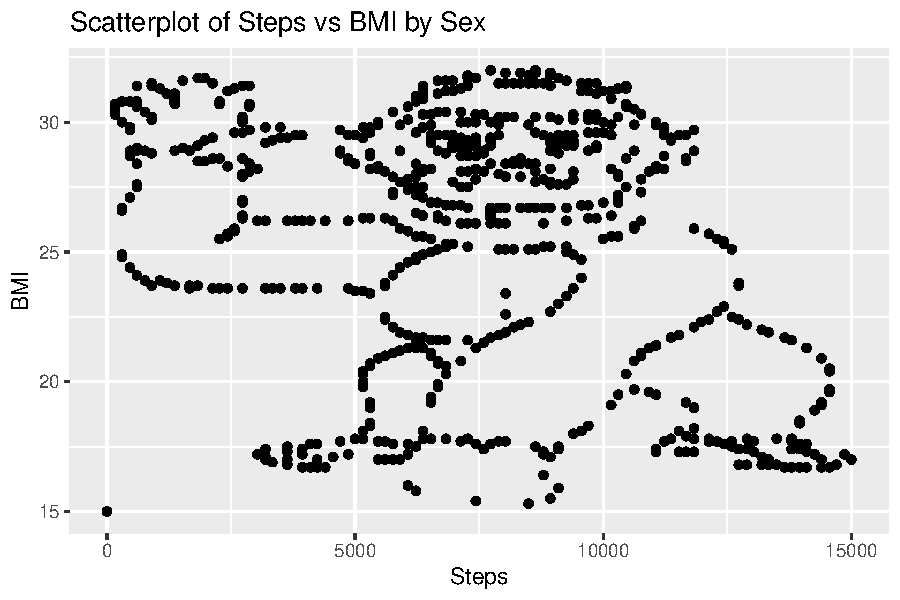
\includegraphics{_main_files/figure-latex/unnamed-chunk-18-1.pdf}

\begin{Shaded}
\begin{Highlighting}[]
\FunctionTok{ggplot}\NormalTok{(male, }\FunctionTok{aes}\NormalTok{(}\AttributeTok{x =}\NormalTok{ steps, }\AttributeTok{y =}\NormalTok{ bmi)) }\SpecialCharTok{+}
  \FunctionTok{geom\_point}\NormalTok{() }\SpecialCharTok{+}
  \FunctionTok{labs}\NormalTok{(}\AttributeTok{x =} \StringTok{"Steps"}\NormalTok{, }\AttributeTok{y =} \StringTok{"BMI"}\NormalTok{) }\SpecialCharTok{+}
  \FunctionTok{ggtitle}\NormalTok{(}\StringTok{"Scatterplot of Steps vs BMI by Sex"}\NormalTok{) }
\end{Highlighting}
\end{Shaded}

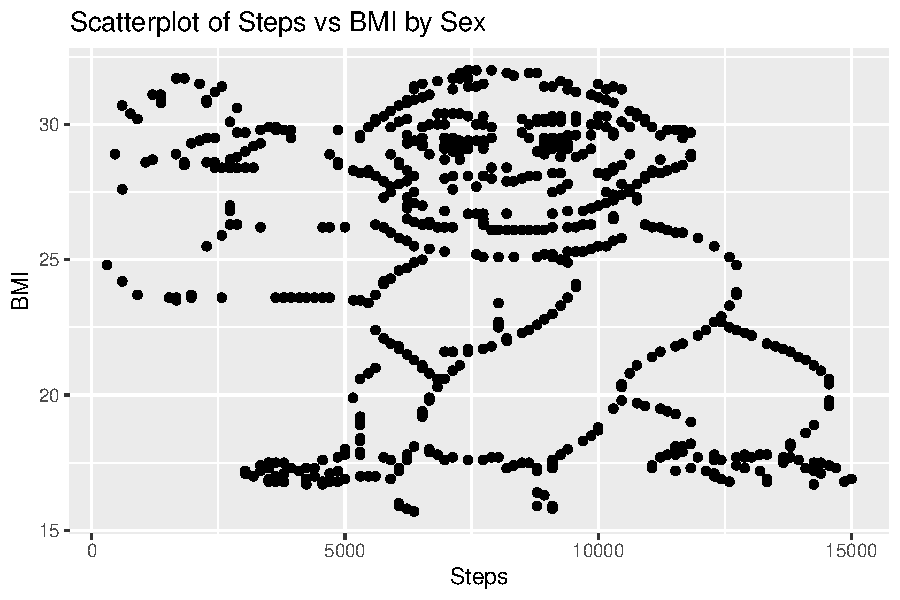
\includegraphics{_main_files/figure-latex/unnamed-chunk-18-2.pdf}

\begin{Shaded}
\begin{Highlighting}[]
\FunctionTok{ggplot}\NormalTok{(all, }\FunctionTok{aes}\NormalTok{(}\AttributeTok{x =}\NormalTok{ steps, }\AttributeTok{y =}\NormalTok{ bmi, }\AttributeTok{color =}\NormalTok{ sex)) }\SpecialCharTok{+}
  \FunctionTok{geom\_point}\NormalTok{() }\SpecialCharTok{+}
  \FunctionTok{labs}\NormalTok{(}\AttributeTok{x =} \StringTok{"Steps"}\NormalTok{, }\AttributeTok{y =} \StringTok{"BMI"}\NormalTok{) }\SpecialCharTok{+}
  \FunctionTok{ggtitle}\NormalTok{(}\StringTok{"Scatterplot of Steps vs BMI by Sex"}\NormalTok{) }\SpecialCharTok{+}
  \FunctionTok{scale\_color\_manual}\NormalTok{(}\AttributeTok{values =} \FunctionTok{c}\NormalTok{(}\StringTok{"F"} \OtherTok{=} \StringTok{"blue"}\NormalTok{, }\StringTok{"M"} \OtherTok{=} \StringTok{"red"}\NormalTok{))  }\CommentTok{\# Optional: Define color mapping}
\end{Highlighting}
\end{Shaded}

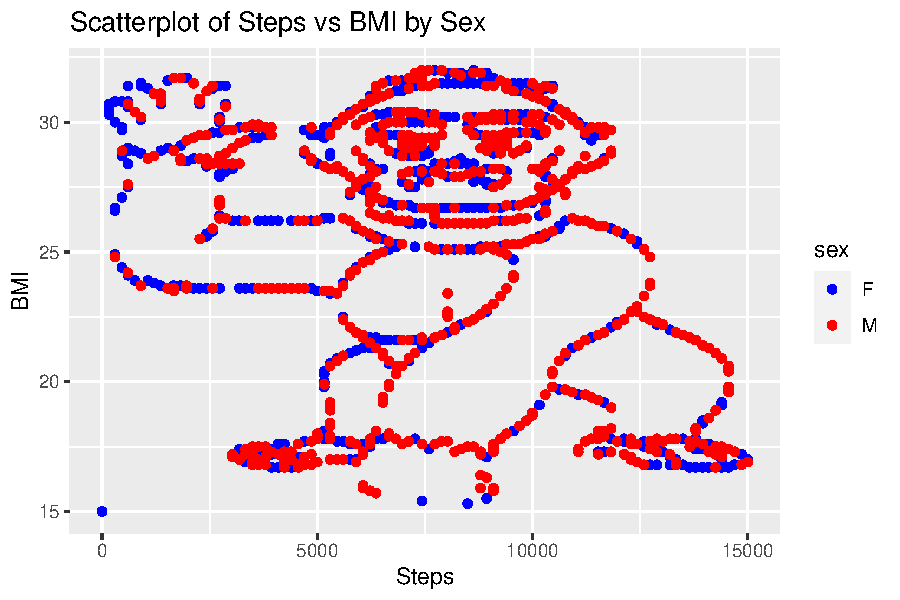
\includegraphics{_main_files/figure-latex/unnamed-chunk-18-3.pdf}

\hypertarget{solution}{%
\section{Solution}\label{solution}}

Will be made available.

\hypertarget{week-2}{%
\chapter{Week 2}\label{week-2}}

\hypertarget{exercise}{%
\section{Exercise}\label{exercise}}

\begin{itemize}
\tightlist
\item
  2nd: simulated dataset and increase the variance: how does that affects the standard error
\end{itemize}

\hypertarget{solution-1}{%
\section{Solution}\label{solution-1}}

\begin{itemize}
\item
  Data taken from \href{https://communities.sas.com/t5/Graphics-Programming/Fun-With-SAS-ODS-Graphics-Don-t-Miss-the-Gorilla-in-the-Data/td-p/697286}{here}.
\item
  Original selective attention, \href{https://www.youtube.com/watch?v=vJG698U2Mvo}{here}.
\item
  Suicide awareness campaign, \href{https://www.youtube.com/watch?v=Lw-YPKR0grk}{here}.
\end{itemize}

\hypertarget{week-3}{%
\chapter{Week 3}\label{week-3}}

\hypertarget{exercise-1}{%
\section{Exercise}\label{exercise-1}}

\hypertarget{solution-2}{%
\section{Solution}\label{solution-2}}

\hypertarget{week-4}{%
\chapter{Week 4}\label{week-4}}

\hypertarget{exercise-2}{%
\section{Exercise}\label{exercise-2}}

\hypertarget{solution-3}{%
\section{Solution}\label{solution-3}}

\hypertarget{week-5}{%
\chapter{Week 5}\label{week-5}}

\hypertarget{exercise-3}{%
\section{Exercise}\label{exercise-3}}

\hypertarget{solution-4}{%
\section{Solution}\label{solution-4}}

\hypertarget{week-6}{%
\chapter{Week 6}\label{week-6}}

\hypertarget{exercise-4}{%
\section{Exercise}\label{exercise-4}}

\hypertarget{solution-5}{%
\section{Solution}\label{solution-5}}

\hypertarget{week-7}{%
\chapter{Week 7}\label{week-7}}

\hypertarget{exercise-5}{%
\section{Exercise}\label{exercise-5}}

\hypertarget{solution-6}{%
\section{Solution}\label{solution-6}}

\hypertarget{week-8}{%
\chapter{Week 8}\label{week-8}}

\hypertarget{exercise-6}{%
\section{Exercise}\label{exercise-6}}

\hypertarget{solution-7}{%
\section{Solution}\label{solution-7}}

\hypertarget{week-9}{%
\chapter{Week 9}\label{week-9}}

\hypertarget{exercise-7}{%
\section{Exercise}\label{exercise-7}}

\hypertarget{solution-8}{%
\section{Solution}\label{solution-8}}

\hypertarget{week-10}{%
\chapter{Week 10}\label{week-10}}

\hypertarget{exercise-8}{%
\section{Exercise}\label{exercise-8}}

\hypertarget{solution-9}{%
\section{Solution}\label{solution-9}}

\hypertarget{week-11}{%
\chapter{Week 11}\label{week-11}}

\hypertarget{exercise-9}{%
\section{Exercise}\label{exercise-9}}

\hypertarget{solution-10}{%
\section{Solution}\label{solution-10}}

\hypertarget{week-12}{%
\chapter{Week 12}\label{week-12}}

\hypertarget{exercise-10}{%
\section{Exercise}\label{exercise-10}}

\hypertarget{solution-11}{%
\section{Solution}\label{solution-11}}

\hypertarget{week-13}{%
\chapter{Week 13}\label{week-13}}

\hypertarget{exercise-11}{%
\section{Exercise}\label{exercise-11}}

\hypertarget{solution-12}{%
\section{Solution}\label{solution-12}}

\hypertarget{week-14}{%
\chapter{Week 14}\label{week-14}}

\hypertarget{exercise-12}{%
\section{Exercise}\label{exercise-12}}

\hypertarget{solution-13}{%
\section{Solution}\label{solution-13}}

  \bibliography{book.bib,packages.bib}

\end{document}
